\subsection{Richardson Extrapolation}
    Quantity of interest $G$ is discretized by some grid-spacing $h$ (Compuer).
    $G \approx G(h)$. Since $h \ll 1$ and $G(h) \xrightarrow{h \rightarrow 0} G$ we can expand G(h) using a Taylor series.
    \begin{equation*}
        G(h) = G(0) +c_1 h +c_2 h^2 + \dots
    \end{equation*}
    $c_i$ constants obtained from the expansion $\leftrightarrow$ Error terms we wish to eliminate. Taylor exapnsion of $G(h/2)$: 
    \begin{equation*}
        G(h/2) = G + \frac{1}{2}c_1 h + \frac{1}{4}c_2 h^2 + \dots
    \end{equation*}
    subtracting these two equations yields:
    \begin{equation*}
        G_1(h) = 2G(h/2) - G(h) = G + c_2' h^2 + c_3' h^3 + \dots
    \end{equation*}
    Leading error term order $h^2 \Rightarrow G_1(h)$ much more accurate than $G(h)$ or $G(h/2)$ for $h\rightarrow 0$ with little added cost. This can be repeated. We can see that $G_n(h) = G + O(h^{n+1})$.
    \begin{equation*}
        \colorboxed{red}{G_n(h) = \frac{1}{2^{n}-1}(2^n G_{n-1}(h/2)-G_{n-1}(h))}
    \end{equation*}
    % \subsubsection{Error estimation}
    \textbf{Error estimation:}
        \begin{equation*}
            \colorboxed{red}{\epsilon(h/2) = G(h/2)-G(h)}
        \end{equation*}
        If $h$ is small this will be a good estimate of the error. If the error is not small enough, then this tells us to keep subdividing.

\subsection{Romberg Integration}
    Improve accuracy of integration by using Richardson's extrapolation. Evalutate Trapeziodal in one interval, two, four, etc. $I_0^1, I_0^2, I_0^4, \dots$ %We start with the trapezoidal rule within a single interval. Then we recalculate within two intervals, four, eigth, etc. $I_0^1, I_0^2, I_0^4, \dots$.
    
    In the calculation of $I_0^n$ for $n$ Intervals, \textbf{half of the needed functions have already been computed earlier}.
    
    Numerical analysis of the error of trapezoidal rule and eliminating leading error term yields
    \begin{gather*}
        I = I_0^n + c_1h^2 + c_2h^4 + c_3 h^6 \\
        \Rightarrow I_0^n = I - c_1 h^2 - c_2h^4 - c_3 h^6\\
    % Evaluate the integral with half the grid size $h_1 = h/2$
    % \begin{equation*}
        I_0^{2n} = I -c_1\frac{h^2}{4} - c_2\frac{h^4}{16} - c_3 \frac{h^6}{64} \\
        \colorboxed{red}{I_k^n = \frac{4^k I_{k-1}^{2n} - I_{k-1}^n}{4^k - 1}}
    \end{gather*}
    % % \end{equation*}
    % eliminating $O(h^2)$ yields
    % \begin{equation*}
    %     I_1^n = \frac{4 I_0^{2n}-I_0^n}{3}= I + \frac{1}{4}c_2h^4 + \dots
    % \end{equation*}
    % General Formula:
    % \end{equation*}
    \begin{center}
        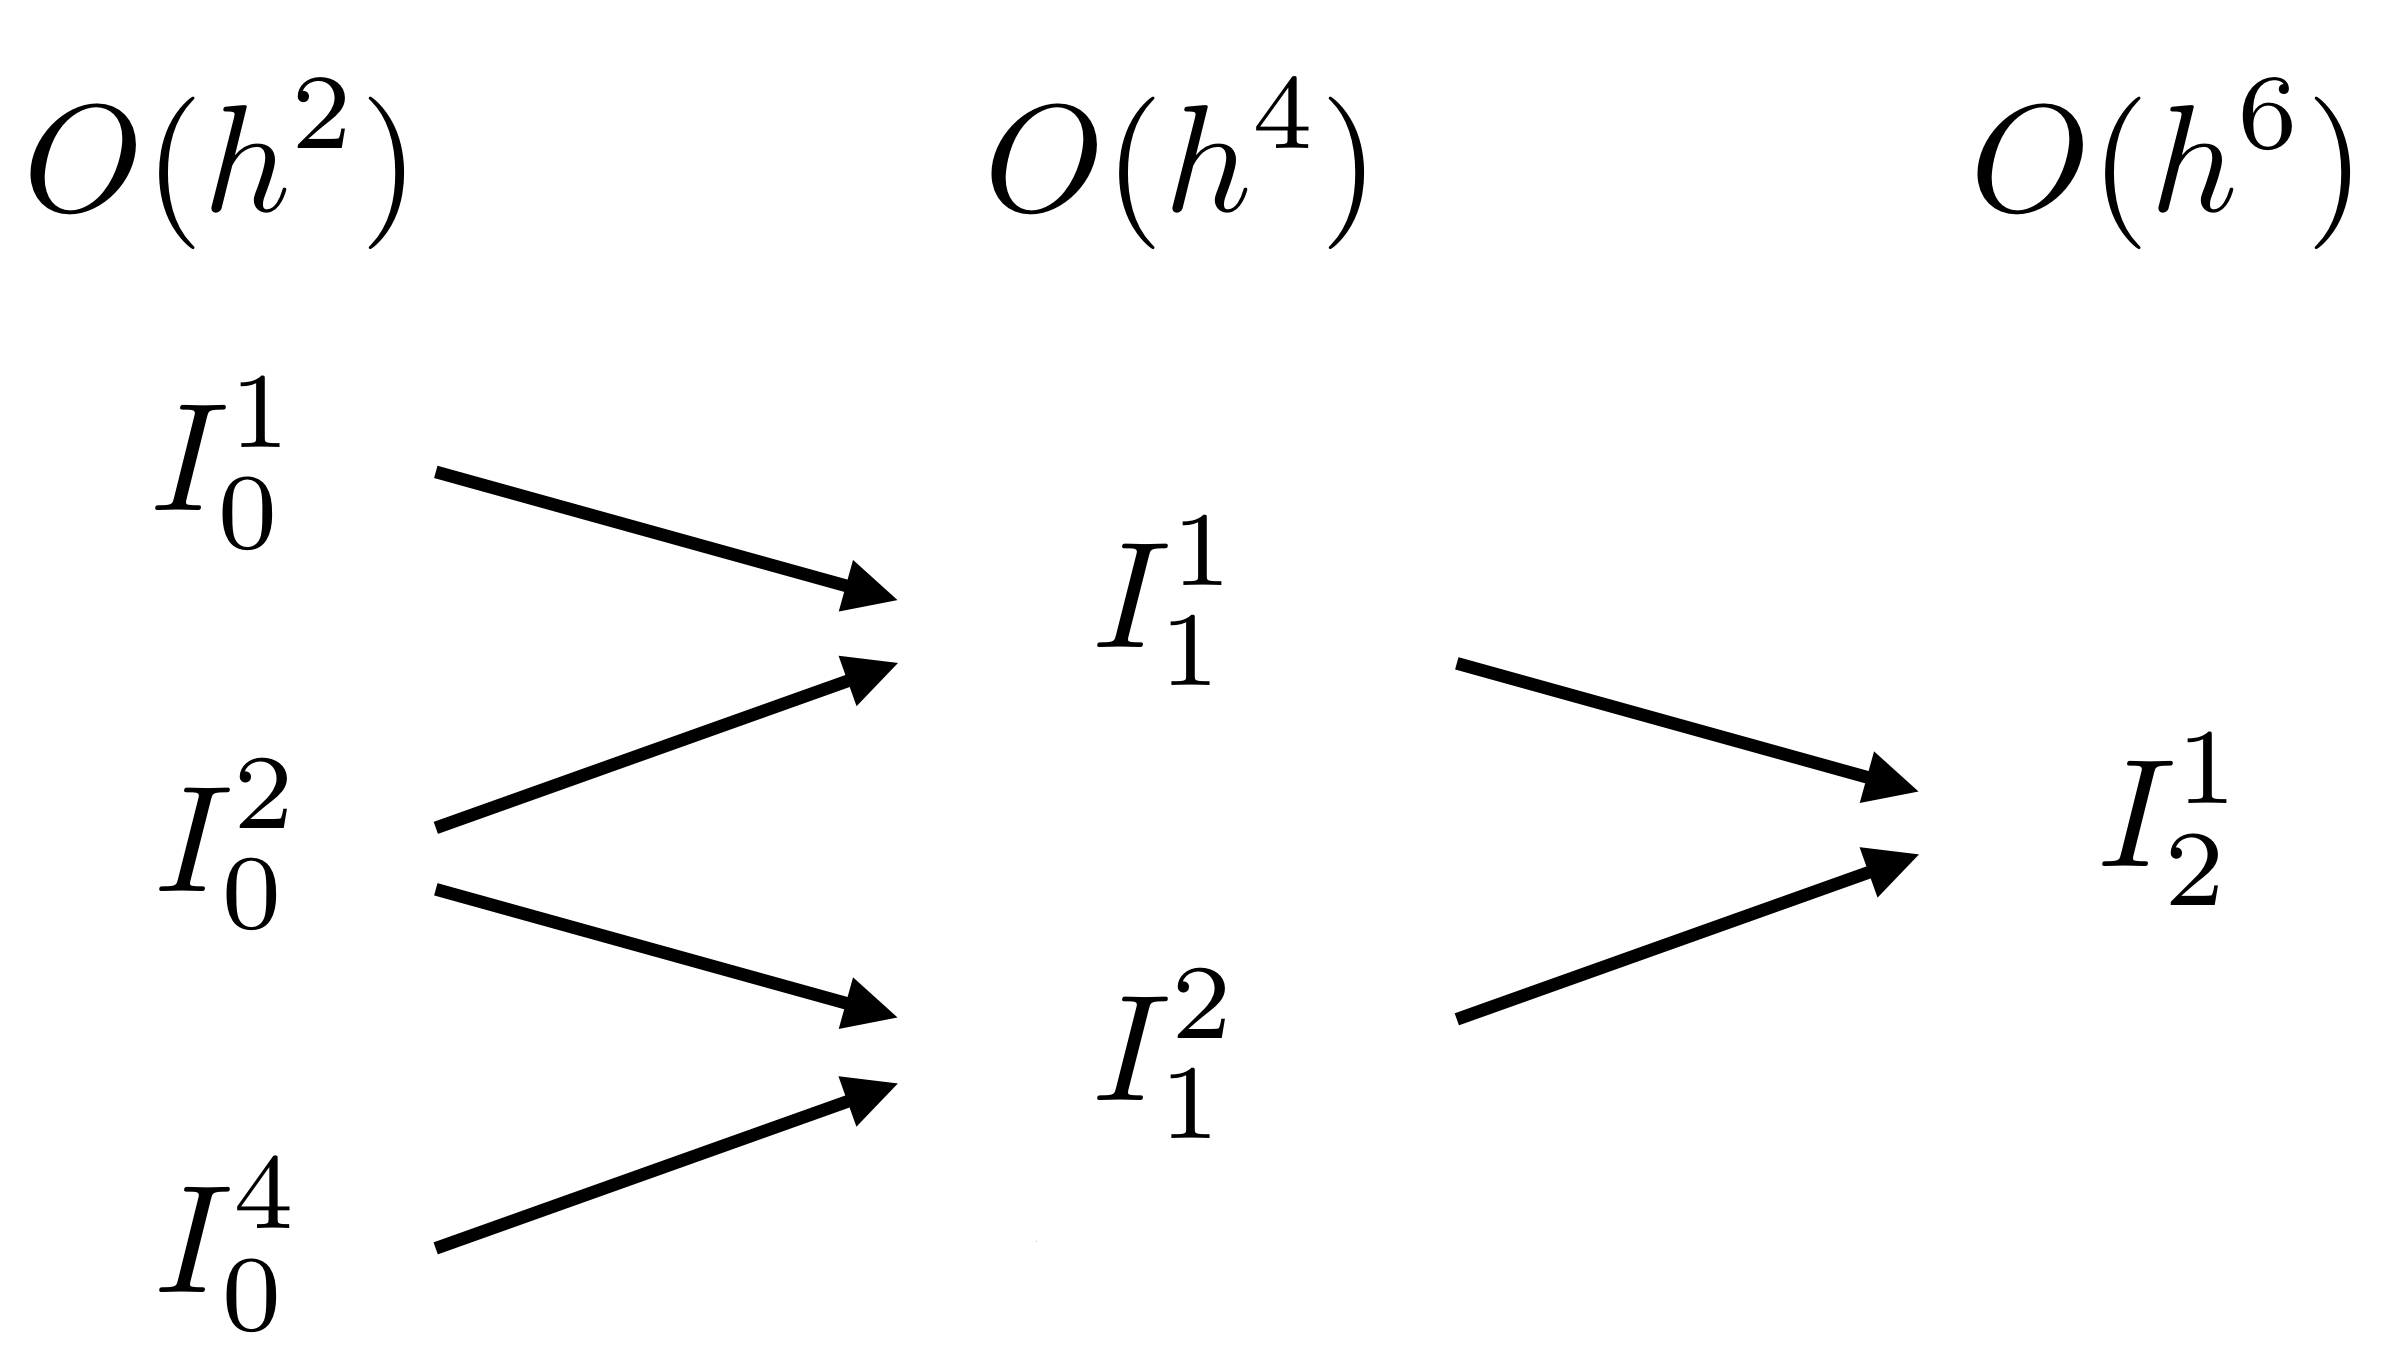
\includegraphics[width = 0.35\linewidth]{images/04/Romberg.jpeg}
        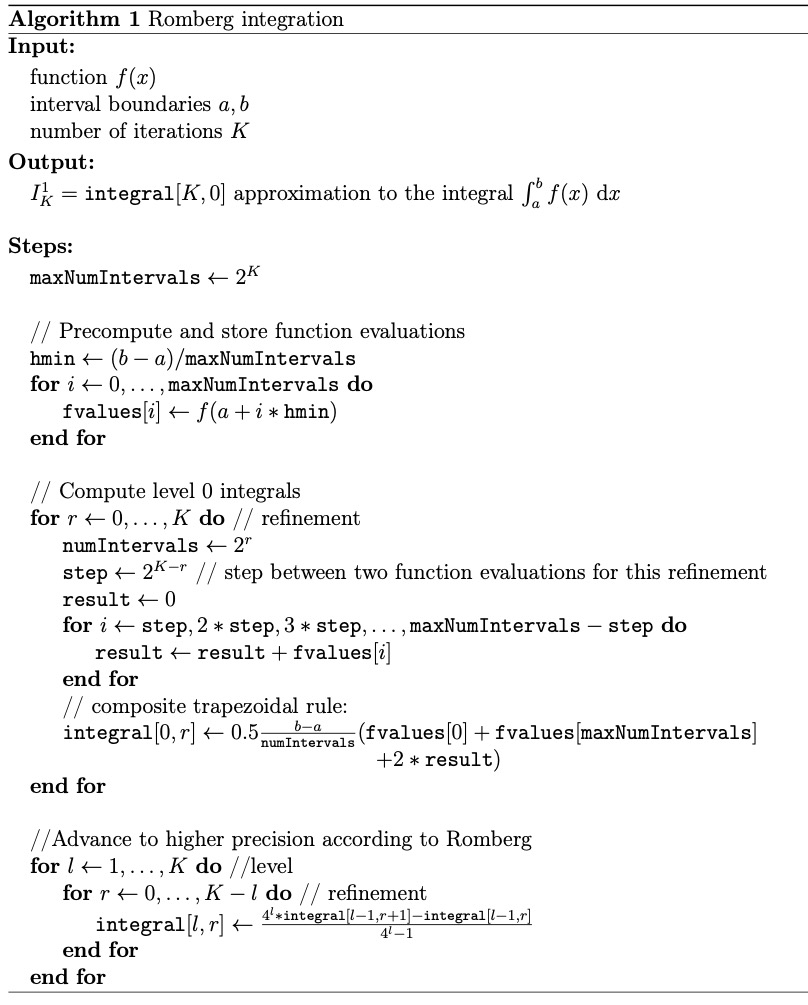
\includegraphics[width = \linewidth, height = 7.84cm]{images/04/Romberg_pseudo.jpg}
    \end{center}